\documentclass[conference]{IEEEtran}
\IEEEoverridecommandlockouts

\usepackage[T1]{fontenc}
\usepackage[utf8]{inputenc}
\usepackage{cite}
\usepackage{amsmath,amssymb}
\usepackage{graphicx}
\usepackage{booktabs}
\usepackage{multirow}
\usepackage{algorithm}
\usepackage{algpseudocode}
\usepackage{listings}
\usepackage{xcolor}
\usepackage{tikz}
\usetikzlibrary{positioning,arrows.meta,shapes.geometric,fit,backgrounds}
\usepackage{microtype}
\usepackage[hidelinks]{hyperref}

% colour-blind safe palette (Okabe--Ito), shared with the plots
\definecolor{cBlue}{HTML}{0072B2}
\definecolor{cOrange}{HTML}{D55E00}
\definecolor{cGreen}{HTML}{009E73}
\definecolor{cGrey}{HTML}{6B6B6B}

\lstset{
  basicstyle=\ttfamily\scriptsize,
  keywordstyle=\color{cBlue}\bfseries,
  commentstyle=\color{cGrey}\itshape,
  numbers=left, numberstyle=\tiny\color{cGrey}, numbersep=4pt,
  frame=single, rulecolor=\color{cGrey!50}, xleftmargin=8pt, framexleftmargin=8pt,
  breaklines=true, showstringspaces=false, columns=fullflexible, language=C++,
  morekeywords={__global__,__restrict__}
}

\algrenewcommand\algorithmicrequire{\textbf{Input:}}
\algrenewcommand\algorithmicensure{\textbf{Output:}}

\begin{document}

\title{Serial versus OpenMP/CUDA Parallel Synthesis of Similarity-Ordered Photo Transition Videos}

\author{\IEEEauthorblockN{1\textsuperscript{st} Awwab Wadekar}
\IEEEauthorblockA{\textit{Dept. of Computer Engineering and Information Technology} \\
\textit{Veermata Jijabai Technological Institute (VJTI)}\\
Mumbai, India \\
aswadekar\_b24@it.vjti.ac.in}
\and
\IEEEauthorblockN{2\textsuperscript{nd} Taha Valiji}
\IEEEauthorblockA{\textit{Dept. of Computer Engineering and Information Technology} \\
\textit{Veermata Jijabai Technological Institute (VJTI)}\\
Mumbai, India \\
tmvaliji\_b24@it.vjti.ac.in}
\and
\IEEEauthorblockN{Mentor: Dr. Sandip Tukaram Shingade}
\IEEEauthorblockA{\textit{Dept. of Computer Engineering and Information Technology} \\
\textit{Veermata Jijabai Technological Institute (VJTI)}\\
Mumbai, India \\
stshingade@it.vjti.ac.in}
}

\maketitle

\begin{abstract}
Turning an unordered folder of photographs into a smooth slideshow video requires three costly steps: extracting a descriptor from every image, arranging the images so that neighbours look alike, and synthesising and encoding many intermediate transition frames. We present a complete pipeline for this task and implement it first twice from the same source: a single-threaded CPU version and a parallel version that uses OpenMP for feature extraction and similarity computation and CUDA for frame blending; we then extend the parallel version in two further steps. Images are described by 3-D HSV colour histograms, compared with histogram correlation, ordered by a greedy nearest-neighbour tour, and joined by cross-dissolve frames. We benchmark the first two versions on five class-balanced subsets (100--1000 images) of a public landscape dataset, at four output resolutions (up to $1920\times1080$) and three transition lengths, giving 120 timed runs on a 16-thread CPU with an RTX~4050 GPU. The parallel stages are substantially faster: against a strictly single-threaded baseline, feature extraction is $7.9\times$ faster on average (up to $9.2\times$) and similarity computation and ordering $7.5\times$ (up to $8.8\times$). The end-to-end speedup, however, is only $1.04$--$1.15\times$ (mean $1.12\times$), because writing the video through a sequential software encoder accounts for $91$--$98\%$ of the serial run time. We quantify this Amdahl-type limit and identify encoder-side parallelism as the necessary next step. We then overlap GPU blending with encoding through a producer--consumer queue and CUDA streams; this gives a further $1.07\times$ (mean over 60 re-run configurations, $1.01$--$1.15\times$), for $1.19\times$ over the serial build, and measurements of GPU and CPU load confirm that a single encoder thread remains the limit. Encoding independent video segments concurrently and joining them without re-encoding removes that limit: with 12 segments the end-to-end speedup rises to $6.55\times$ over the serial build (mean $6.3\times$ per configuration, $5.3\times$ over the queue build) at a parallel efficiency of $0.41$ on 16 threads. Restricting the same pipeline to six threads gives $5.3\times$ at an efficiency of $0.88$ and a cost of only $1.13\times$ the serial cost, i.e.\ nearly cost-optimal, whereas the 16-thread build costs $2.4\times$ and the first two parallel builds $13$--$14\times$. An OpenMP thread-scaling study shows that this CPU caps a CPU-bound stage at about $8.4\times$ (efficiency $0.84$ on the $10$ physical cores), so the 16-thread build reaches about $78\%$ of what the machine can deliver. Independent concurrent encodes of the same video, without GPU, queue or join, scale to only $7.2\times$ on 16 copies, and the segmented pipeline reaches $94\%$ (12 segments) and $98\%$ (six threads) of the corresponding encoder capacity, so the remaining gap to ideal is the encoder and the CPU rather than our pipeline. We also found that OpenCV's own thread pool had made the original serial baseline up to $1.5\times$ faster in feature extraction than a strictly single-threaded one, and we repeated the serial sweep with the pool disabled.
\end{abstract}

\begin{IEEEkeywords}
parallel computing, OpenMP, CUDA, image similarity, colour histograms, video generation, frame interpolation, producer--consumer queue, CUDA streams, parallel efficiency, cost optimality, speedup analysis
\end{IEEEkeywords}

%=====================================================================
\section{Introduction}
Personal and online photo collections are large and usually unordered. Presenting them as a video, where each photograph dissolves smoothly into the next, is a common request, but it is computationally heavy: every image must be decoded and analysed, every pair of images compared in order to choose a pleasing sequence, and tens of thousands of transition frames rendered and compressed. The work is also naturally parallel in most of its stages, which makes it a good case study for comparing a serial implementation with a CPU--GPU parallel one.

Our design draws on three lines of earlier work. Snavely \emph{et al.}\ presented a system for browsing large, unstructured photo collections that uses image-based rendering to \emph{smoothly transition between photographs} \cite{snavely2006}; we adopt this setting of turning an unordered photo set into a continuous visual sequence. Niklaus \emph{et al.}\ cast video frame interpolation as a (separable) convolution applied to a pair of input frames, and note that per-pixel 2-D kernels become very memory-hungry at 1080p (26\,GB for $41\times41$ kernels), which motivates their separable, whole-frame formulation \cite{niklaus2017}. Fan \emph{et al.}\ (Co-ViA) observed that in learned interpolation one stage---optical-flow estimation, over $60\%$ of run time in the baseline they analyse---dominates, and obtained large gains only by restructuring the pipeline around that bottleneck \cite{fan2024}. We use the first as the application setting, the second as the interpolation viewpoint (in its simplest, learning-free form: a per-pixel blend of two frames), and the third as the methodological lesson that the benefit of accelerating any stage is bounded by the share of the stages that remain unchanged.

\textbf{Contributions.} (i) A complete, reproducible serial and a parallel (OpenMP\,+\,CUDA) implementation of an image-to-video transition pipeline sharing identical algorithms and parameters; (ii) a command-line and JSON-driven benchmarking harness that sweeps datasets, resolutions and transition lengths and records per-stage timings; (iii) a 120-run measurement study with a stage-level analysis explaining why large stage speedups translate into a modest end-to-end gain; (iv) a producer--consumer extension that overlaps GPU blending with encoding, evaluated over a further 60 runs, together with a utilisation analysis of what still limits it; (v) concurrent encoding of independent video segments, a six-thread variant, and a master comparison of all builds using speedup, efficiency, cost and the Amdahl and Karp--Flatt metrics; (vi) an OpenMP thread-scaling study and an independent-encoder scaling test that give measured hardware ceilings, and that expose a threading effect in the original serial baseline, which we corrected by repeating the serial sweep.

\textbf{Organisation.} Section~II states the problem. Section~III describes the approach and algorithms, Section~IV their implementation, and Section~V the datasets and experimental procedure. Results are reported in Section~VI and analysed in Section~VII. Section~VIII presents and evaluates the producer--consumer extension that overlaps blending with encoding, and Section~IX the parallel-segment extension. Section~X compares all builds, including parallel efficiency, cost optimality and the classical Amdahl, Karp--Flatt and Gustafson views, reports the thread- and encoder-scaling studies and the final six-thread comparison; Section~XI concludes.

%=====================================================================
\section{Problem Statement}
Given a directory of $N$ images $\mathcal{I}=\{I_1,\dots,I_N\}$ of arbitrary sizes, an output resolution $W\times H$ and a number $F\ge 0$ of intermediate frames per image pair, produce a single video that (a) shows every image exactly once, (b) orders the images so that consecutive images are as visually similar as possible, and (c) inserts $F$ synthesised frames between consecutive images so that one image fades into the next. The video contains
\begin{equation}
  T = (N-1)(F+1) + 1
  \label{eq:frames}
\end{equation}
frames. We want to know:
\begin{enumerate}
  \item How much faster can each stage be made by CPU multithreading (OpenMP) and GPU offload (CUDA) compared with an equivalent single-threaded implementation?
  \item How do the speedups depend on the dataset size $N$, the resolution $W\times H$, and the transition length $F$?
  \item Which stage limits the end-to-end speedup, and by how much?
  \item Once that stage is attacked, how efficient and how cost-optimal is the resulting parallel system, and how much of the remaining gap is the algorithm, our implementation, or the hardware?
\end{enumerate}
Ordering the images optimally is a travelling-salesman-type problem; we do not seek the optimum but a cheap, deterministic heuristic that is identical in both implementations, so that the comparison isolates the effect of parallelisation.

%=====================================================================
\section{Approach and Algorithms}

\subsection{Pipeline overview}
The pipeline (Fig.~\ref{fig:pipeline}) has five stages. Stages~1 and~2 are data-parallel across images and image pairs; Stage~3 is a short sequential scan; Stage~4 is data-parallel across pixels; Stage~5 is, in the first version, a sequential stream into the video encoder (Sections~\ref{sec:queue} and~\ref{sec:segments} change Stages~4 and~5).

\begin{figure*}[t]
\centering
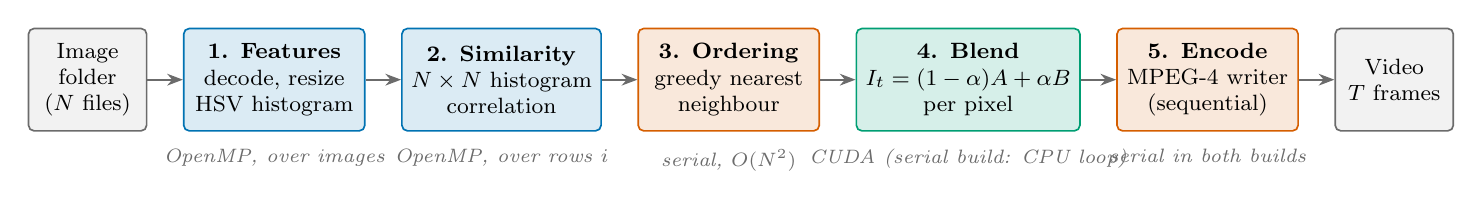
\begin{tikzpicture}[
  node distance=4mm and 4.5mm,
  blk/.style={draw, rounded corners=2pt, minimum height=13mm, minimum width=23mm, align=center, font=\footnotesize, line width=0.6pt},
  par/.style={blk, fill=cBlue!14, draw=cBlue},
  gpu/.style={blk, fill=cGreen!16, draw=cGreen},
  seq/.style={blk, fill=cOrange!14, draw=cOrange},
  io/.style={blk, fill=black!5, draw=cGrey, minimum width=15mm},
  tag/.style={font=\scriptsize\itshape, text=cGrey},
  arr/.style={-{Stealth[length=2mm]}, line width=0.6pt, draw=cGrey}
]
\node[io] (in) {Image\\folder\\($N$ files)};
\node[par, right=of in] (s1) {\textbf{1. Features}\\decode, resize\\HSV histogram};
\node[par, right=of s1] (s2) {\textbf{2. Similarity}\\$N\times N$ histogram\\correlation};
\node[seq, right=of s2] (s3) {\textbf{3. Ordering}\\greedy nearest\\neighbour};
\node[gpu, right=of s3] (s4) {\textbf{4. Blend}\\$I_t=(1-\alpha)A+\alpha B$\\per pixel};
\node[seq, right=of s4] (s5) {\textbf{5. Encode}\\MPEG-4 writer\\(sequential)};
\node[io, right=of s5] (out) {Video\\$T$ frames};
\foreach \a/\b in {in/s1,s1/s2,s2/s3,s3/s4,s4/s5,s5/out} \draw[arr] (\a) -- (\b);
\node[tag, below=1mm of s1] {OpenMP, over images};
\node[tag, below=1mm of s2] {OpenMP, over rows $i$};
\node[tag, below=1mm of s3] {serial, $O(N^2)$};
\node[tag, below=1mm of s4] {CUDA (serial build: CPU loop)};
\node[tag, below=1mm of s5] {serial in both builds};
\end{tikzpicture}
\caption{Pipeline stages and where parallelism is applied. Blue: parallelised on the CPU; green: parallelised on the GPU; orange: sequential in both builds. In the serial build every stage runs single-threaded on the CPU. The figure shows the first version; Sections~\ref{sec:queue} and~\ref{sec:segments} overlap Stage~4 with Stage~5 and parallelise Stage~5.}
\label{fig:pipeline}
\end{figure*}

\subsection{Image descriptor: HSV colour histogram}
Each image is resized to the output resolution $W\times H$ (bilinear interpolation) and converted from BGR to HSV, a colour space in which hue is separated from brightness and is therefore more stable under lighting change than raw RGB. A three-dimensional histogram with $16$ hue ($[0,180)$), $8$ saturation and $8$ value bins ($[0,256)$ each) is computed, giving a descriptor of $16\cdot 8\cdot 8=1024$ bins, which is then min--max normalised to $[0,1]$. Colour-histogram matching is a classical, inexpensive way of comparing images \cite{swain1991}; it is robust to small viewpoint changes, which suits photographs of the same scene type.

\subsection{Pairwise similarity}
For histograms $H_i, H_j$ with means $\bar H_i,\bar H_j$ over the $B=1024$ bins, similarity is the Pearson correlation
\begin{equation}
  s_{ij}=\frac{\sum_{b}(H_i(b)-\bar H_i)(H_j(b)-\bar H_j)}
  {\sqrt{\sum_{b}(H_i(b)-\bar H_i)^2\;\sum_{b}(H_j(b)-\bar H_j)^2}},
  \label{eq:corr}
\end{equation}
(OpenCV's \texttt{HISTCMP\_CORREL}). Because $s_{ij}=s_{ji}$, only the upper triangle is computed and mirrored: $N(N-1)/2$ comparisons of cost $O(B)$ each.

\subsection{Ordering}
The images are sequenced by the greedy nearest-neighbour rule of Algorithm~\ref{alg:order}: start at the first image, and repeatedly move to the not-yet-visited image with the highest correlation to the current one. It costs $O(N^2)$, is deterministic, and is identical in the serial and parallel builds. It gives no optimality guarantee, and we do not evaluate the visual quality of the resulting order.

\begin{algorithm}[t]
\caption{Greedy similarity ordering}
\label{alg:order}
\begin{algorithmic}[1]
\Require similarity matrix $S\in\mathbb{R}^{N\times N}$
\Ensure permutation $\pi$ of $\{1,\dots,N\}$
\State $\pi \gets [1]$;\; $\textit{visited}[1]\gets \textbf{true}$;\; $c \gets 1$
\For{$k=2$ \textbf{to} $N$}
  \State $n \gets \arg\max_{j:\,\neg\textit{visited}[j]} S_{cj}$
  \State append $n$ to $\pi$;\; $\textit{visited}[n]\gets\textbf{true}$;\; $c\gets n$
\EndFor
\State \Return $\pi$
\end{algorithmic}
\end{algorithm}

\subsection{Transition synthesis}
For consecutive images $A=I_{\pi_k}$ and $B=I_{\pi_{k+1}}$ the $f$-th intermediate frame ($f=1,\dots,F$) is the cross-dissolve
\begin{equation}
  I_f(x,y,c)=\big\lfloor (1-\alpha_f)\,A(x,y,c)+\alpha_f\,B(x,y,c)\big\rfloor,
  \label{eq:blend}
\end{equation}
with $\alpha_f=f/(F+1)$, for every pixel $(x,y)$ and channel $c$. This is the simplest instance of the ``combine two frames with a per-pixel weighting'' idea behind convolution-based interpolation \cite{niklaus2017}, with a constant, content-independent kernel and no motion estimation; it therefore handles the unrelated pairs in a photo collection (which have no meaningful motion) at a cost of two multiplies and one add per byte. Each pixel and channel is independent, which makes the stage embarrassingly parallel. Frames are written in order, $A$ first and the last image at the end, giving Eq.~\eqref{eq:frames} frames at $60$\,fps.

\subsection{Parallelisation strategy}
Table~\ref{tab:strategy} summarises how each stage is mapped. Stages~1 and~2 use \emph{data parallelism with dynamic scheduling}: image decode times differ, and the triangular loop in Stage~2 gives early rows more work than late rows. Stage~4 uses one GPU thread per pixel. In this first version, Stage~5 is not parallelised across frames with the software encoder used here, because frames must be appended in order; Section~\ref{sec:segments} later circumvents this by encoding independent segments and joining them.

\begin{table}[t]
\caption{Mapping of stages to execution resources in the first parallel build (P$_1$)}
\label{tab:strategy}
\centering
\footnotesize
\begin{tabular}{@{}llll@{}}
\toprule
Stage & Work items & Serial build & Parallel build \\
\midrule
1 Features & $N$ images & loop & OpenMP, dynamic \\
2 Similarity & $N(N{-}1)/2$ pairs & loop & OpenMP, dynamic \\
3 Ordering & $N$ steps & loop & loop (same) \\
4 Blend & $W{\cdot}H{\cdot}3$ bytes/frame & CPU loop & CUDA kernel \\
5 Encode & $T$ frames & sequential & sequential \\
\bottomrule
\end{tabular}
\end{table}

%=====================================================================
\section{Implementation}

\subsection{Code organisation and build}
\label{sec:impl-baseline}
The code base is C++17 with CUDA. Three executables are built by one CMake project (Release configuration by default, so that timings reflect optimised code):
\begin{itemize}
  \item \texttt{pipeline\_parallel}: \texttt{main.cpp} + \texttt{kernels.cu} + \texttt{blocking\_queue.hpp}, linked against OpenCV, OpenMP and the CUDA runtime.
  \item \texttt{pipeline\_serial}: \texttt{main\_serial.cpp}, linked against OpenCV only; it contains no OpenMP pragma and no CUDA call, so it is a single-threaded baseline in our own code (in the first sweep OpenCV's internal thread pool was nevertheless active in it; the final serial sweep disables it with \texttt{--cv-threads 1}, see Section~\ref{sec:threads}).
  \item \texttt{encode\_bench}: \texttt{encode\_bench.cpp}, linked against OpenCV only; a small benchmark that runs several independent encodes at once (Section~\ref{sec:threads}).
\end{itemize}
The three parallel builds studied below are successive states of \texttt{pipeline\_parallel}: P$_1$ is the synchronous implementation of the first version (an earlier revision in the repository history), P$_2$ is the current code with \texttt{--segments 1}, and P$_3$ is the current code with \texttt{--segments} $K>1$, which also needs the \texttt{ffmpeg} executable.
A shared header, \texttt{common.hpp}, contains everything that must be identical in both builds---argument parsing, image listing, the HSV histogram, and the greedy ordering of Algorithm~\ref{alg:order}---so differences in run time come only from how the stages are executed.

\subsection{Command-line interface}
Both programs take named, order-independent options: \texttt{--dataset}, \texttt{--width}/\texttt{--height} (accepted only together; default $1280\times720$), \texttt{--frames} (default $30$), \texttt{--output}, and \texttt{--metrics}, which writes the stage timings as JSON. Invalid values (non-positive sizes, only one of width/height, unknown or positional arguments) are rejected with exit code~2. The parallel build additionally takes \texttt{--segments} (concurrent video segments, Section~\ref{sec:segments}) and \texttt{--threads} (OpenMP threads); both builds accept \texttt{--cv-threads}, the size of OpenCV's internal thread pool.

\subsection{Parallel stages}
Stage~1 is a single \texttt{\#pragma omp parallel for schedule(dynamic)} over the image list: each thread decodes, resizes and histograms its own images and writes only to its own slots of the pre-allocated arrays, so no locking is needed. Stage~2 uses the same pragma over the row index $i$ of the upper triangle, each iteration computing $s_{ij}$ for $j>i$ and writing both $S_{ij}$ and $S_{ji}$ (distinct elements, hence race-free). Images that fail to decode are dropped before Stage~2. The ordering (Stage~3) runs on one thread in both builds.

\subsection{GPU blending}
In the first parallel build (P$_1$), for each consecutive pair the two images are copied to the device once, and each of the $F$ intermediate frames is produced by a kernel launch followed by a device-to-host copy into a reusable frame buffer that is handed to the encoder. The kernel assigns one thread to one pixel (three bytes), with $256$ threads per block (Listing~\ref{lst:kernel}); the host wrapper synchronises after each launch (removed in P$_2$, Section~\ref{sec:queue}).

\begin{lstlisting}[caption={CUDA blend kernel (Eq.~\eqref{eq:blend}).},label={lst:kernel},float=t]
__global__ void blendKernel(const unsigned char* __restrict__ A,
                            const unsigned char* __restrict__ B,
                            unsigned char* __restrict__ out,
                            float alpha, int totalPixels) {
  int idx = blockDim.x * blockIdx.x + threadIdx.x;
  if (idx < totalPixels) {
    int p = idx * 3;                      // B, G, R
    float inv = 1.0f - alpha;
    out[p+0] = (unsigned char)(A[p+0]*inv + B[p+0]*alpha);
    out[p+1] = (unsigned char)(A[p+1]*inv + B[p+1]*alpha);
    out[p+2] = (unsigned char)(A[p+2]*inv + B[p+2]*alpha);
  }
}
\end{lstlisting}

The serial build uses the same expression in a plain loop over the $W\cdot H\cdot 3$ bytes of the frame, with the same truncation.

\subsection{Video encoding}
In the first version both builds stream frames directly into an OpenCV \texttt{VideoWriter} using the MPEG-4 Part~2 (\texttt{mp4v}) codec at $60$\,fps; no frame is stored beyond the one being encoded. The reported ``blend + encode'' time therefore covers blending (CPU or GPU, including host--device transfers), codec work and file output. All $N$ resized images are held in memory, which costs $N\cdot W\cdot H\cdot 3$ bytes (6.2\,GB for $N{=}1000$ at $1920\times1080$). Sections~\ref{sec:queue} and~\ref{sec:segments} change how frames reach the writer (queue, several writers), not the codec.

\subsection{Benchmark driver}
A Python driver (\texttt{run\_pipeline.py}) configures and builds the project with CMake, then reads a JSON file describing datasets, each with a path, an output path, a list of $(W,H)$ pairs and a list of $F$ values. For every dataset and every combination it runs the serial and then the parallel executable (or only one of them, with \texttt{--mode}); it passes \texttt{--segments}, \texttt{--threads} and \texttt{--cv-threads} on to the executables and records them in the CSV file. The driver validates its input and \emph{reports but does not abort on} problems: a missing path, a dataset with fewer than $20$ images, or an invalid setting (e.g.\ a negative height) causes only that dataset or setting to be skipped. Every run's three stage times, total frames and wall time are appended immediately to a CSV file, so a long sweep survives interruptions. To limit disk usage the driver deletes each run's video after its timings are saved, keeping only the $1920\times1080$, $F{=}20$ video of each dataset.

\subsection{Experiment and analysis scripts}
Further experiments use small dedicated scripts, each writing a CSV file: \texttt{run\_segment\_pilot.py} (segment count), \texttt{run\_thread\_scaling.py} (OpenMP threads) and \texttt{run\_encoder\_scaling.py} (independent encodes, using \texttt{encode\_bench}). The scripts \texttt{make\_figures.py}, \texttt{make\_queue\_results.py}, \texttt{make\_segment\_results.py} and \texttt{make\_thread\_results.py} turn the CSV files into the tables and figures of this paper. Code, scripts and raw results are in the project repository.

%=====================================================================
\section{Dataset and Processing}

\subsection{Source data}
We use the public Kaggle dataset ``Landscape Recognition | Image Dataset (12k Images)'' \cite{kaggle_landscape}, a multi-class landscape classification set. Its training split has five classes---Coast, Desert, Forest, Glacier and Mountain---of $2000$ JPEG images each. The source images are small (for example $275\times183$ and $300\times168$), so every output resolution up-samples them; this affects image content but not the amount of computation per pixel, which is what we measure.

\subsection{Subsets}
A setup script samples, with a fixed random seed ($42$), an equal number of images from each class and copies them into flat folders, producing five datasets of $N=100, 200, 500, 750$ and $1000$ images (Table~\ref{tab:datasets}). Class balance ensures that the similarity structure is non-trivial: images of the same class tend to correlate more strongly than images of different classes.

\begin{table}[t]
\caption{Datasets and experimental grid}
\label{tab:datasets}
\centering
\footnotesize
\begin{tabular}{@{}lccc@{}}
\toprule
Dataset & Images $N$ & Per class & Pairs $N(N{-}1)/2$ \\
\midrule
\texttt{landscape\_100}  & 100  & 20  & 4{,}950 \\
\texttt{landscape\_200}  & 200  & 40  & 19{,}900 \\
\texttt{landscape\_500}  & 500  & 100 & 124{,}750 \\
\texttt{landscape\_750}  & 750  & 150 & 280{,}875 \\
\texttt{landscape\_1000} & 1000 & 200 & 499{,}500 \\
\midrule
\multicolumn{4}{@{}p{0.92\columnwidth}@{}}{Resolutions: $640{\times}360$, $1024{\times}768$, $1280{\times}720$, $1920{\times}1080$. Transition lengths $F\in\{10,20,30\}$. Modes: serial, parallel. Total: $5\times4\times3\times2=120$ runs.} \\
\bottomrule
\end{tabular}
\end{table}

\subsection{Experimental procedure and platform}
Every dataset is run with every resolution and every $F$ in both modes (120 runs, all completed successfully). The driver is executed once, sequentially, so serial and parallel runs never compete for the machine. Timings are taken inside the executables with a monotonic clock and cover three stages: \emph{feature extraction} (Stage~1, including image decoding), \emph{similarity and ordering} (Stages~2--3), and \emph{blend + encode} (Stages~4--5); the \emph{pipeline time} is their sum and excludes process start-up and file listing. The platform is a laptop with an Intel Core i5-13450HX CPU ($10$ cores, $16$ hardware threads), $31$\,GB RAM, and an NVIDIA GeForce RTX~4050 Laptop GPU; software is Linux, GCC~16.2, OpenCV~5.0 \cite{bradski2000}, OpenMP \cite{dagum1998} with the default of $16$ threads, and CUDA~13.4 \cite{nickolls2008}. The serial runs of the results below were repeated with OpenCV's internal thread pool disabled (\texttt{--cv-threads 1}), so that the serial baseline is strictly single-threaded (Section~\ref{sec:threads}); the parallel builds keep OpenCV's default pool. Table~\ref{tab:experiments} lists all experiments; each sweep was executed alone on the machine.

\begin{table*}[t]
\caption{Overview of all experiments (27--28 October). Sweeps use the grid of Table~\ref{tab:datasets}; each run was executed once unless repetitions are stated. Utilisation samples (\texttt{nvidia-smi}, \texttt{top}) were taken during E2 and E3, and output checks are described in Sections~\ref{sec:queue} and~\ref{sec:segments}.}
\label{tab:experiments}
\centering
\footnotesize
\begin{tabular}{@{}lp{0.6\textwidth}rl@{}}
\toprule
ID & Experiment & Runs & Time \\
\midrule
E1 & First sweep: serial (OpenCV default pool) and P$_1$, $60$ configurations each; the serial part is superseded by E7 & 120 & 27 Oct, 17:46--19:40 \\
E2 & P$_2$ (queue) sweep & 60 & 27 Oct, 22:06--22:57 \\
E3 & P$_3$ sweep, $K{=}12$ segments, $16$ threads & 60 & 27 Oct, 23:08--23:18 \\
E4 & Segment-count pilot, $K\in\{1,2,4,6,8,12,16\}$, three interleaved repetitions & 21 & -- \\
E5 & OpenMP thread scaling, $t\in\{1,2,4,6,8,10,12,16\}$, four configurations, three repetitions, plus serial with OpenCV pool off and at default & 120 & -- \\
E6 & Independent concurrent encodes, $1$--$16$ copies, three repetitions & 24 & -- \\
E7 & Serial re-run, OpenCV pool disabled (\texttt{--cv-threads 1}) & 60 & 28 Oct, 00:19--01:19 \\
E8 & P$_3$ with six threads (\texttt{--threads 6 --segments 6}) & 60 & 28 Oct, 00:07--00:19 \\
\bottomrule
\end{tabular}
\end{table*}

\subsection{Output consistency}
In a preliminary check on a separate $233$-image folder at $640\times360$ with $F{=}2$, both builds produced videos with the same number of frames ($697$, as predicted by Eq.~\eqref{eq:frames}); after lossy MPEG-4 encoding, decoded frames differed by a mean absolute value of $0.52$ intensity levels (out of $255$; largest per-frame mean $1.41$). We therefore regard the two outputs as visually equivalent, and did not otherwise evaluate image quality.

%=====================================================================
\section{Results}
In Sections~\ref{sec:impl-baseline}--VII, ``serial'' (S) is the strictly single-threaded baseline (E7) and ``parallel'' (P) is the first parallel build P$_1$ (E1); the later builds P$_2$ and P$_3$ are introduced in Sections~\ref{sec:queue} and~\ref{sec:segments}.

\subsection{Stage-level times}
Table~\ref{tab:main} gives the per-stage times of both builds at $1920\times1080$ and $F{=}20$ for every dataset. Fig.~\ref{fig:breakdown} shows the same breakdown graphically at three resolutions: in both builds the blend-and-encode stage is almost the entire bar.

\begin{table*}[t]
\caption{Stage times (ms), serial (S) versus parallel (P), at $1920\times1080$, $F=20$. Speedup $=$ pipeline S / pipeline P.}
\label{tab:main}
\centering
\footnotesize
\setlength{\tabcolsep}{4.2pt}
\begin{tabular}{@{}rr rr rr rr rr r@{}}
\toprule
 & & \multicolumn{2}{c}{Feature extraction} & \multicolumn{2}{c}{Similarity + order} & \multicolumn{2}{c}{Blend + encode} & \multicolumn{2}{c}{Pipeline total} & \\
\cmidrule(lr){3-4}\cmidrule(lr){5-6}\cmidrule(lr){7-8}\cmidrule(lr){9-10}
$N$ & Frames $T$ & S & P & S & P & S & P & S & P & Speedup \\
\midrule
100 & 2080 & 711 & 98 & 4 & 1 & 23{,}698 & 21{,}366 & 24{,}413 & 21{,}465 & 1.14 \\
200 & 4180 & 1{,}422 & 211 & 16 & 2 & 47{,}239 & 43{,}586 & 48{,}677 & 43{,}799 & 1.11 \\
500 & 10480 & 3{,}595 & 418 & 102 & 12 & 117{,}992 & 106{,}726 & 121{,}689 & 107{,}156 & 1.14 \\
750 & 15730 & 5{,}389 & 654 & 223 & 26 & 177{,}304 & 162{,}063 & 182{,}916 & 162{,}743 & 1.12 \\
1000 & 20980 & 7{,}265 & 955 & 398 & 48 & 235{,}999 & 213{,}825 & 243{,}663 & 214{,}828 & 1.13
\\
\bottomrule
\end{tabular}
\end{table*}

\begin{figure*}[t]
\centering
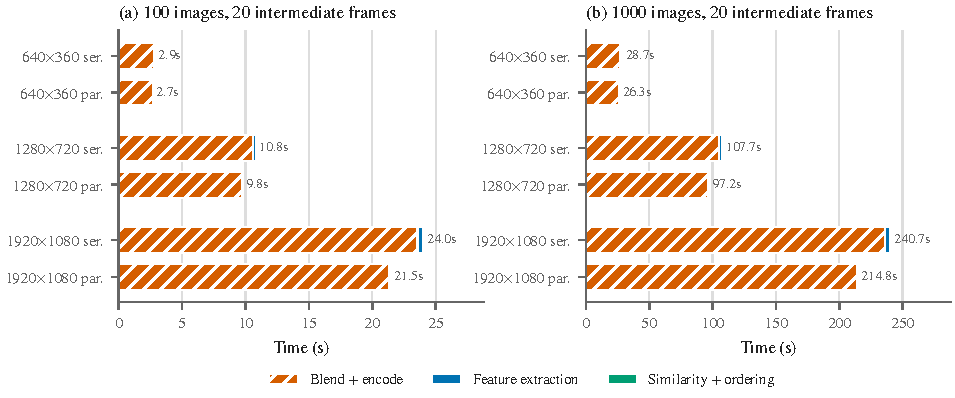
\includegraphics[width=0.96\textwidth]{figures/breakdown.pdf}
\caption{Time breakdown of the serial (ser.) and parallel (par.) builds for $N{=}100$ (a) and $N{=}1000$ (b) at three resolutions, $F{=}20$. Totals are annotated. Feature extraction and similarity/ordering (blue and green) are barely visible next to blend + encode (hatched orange).}
\label{fig:breakdown}
\end{figure*}

\subsection{Parallel-stage speedups}
Fig.~\ref{fig:stagespeedup} shows the speedup of the two parallel CPU stages. Over all 60 configurations (each measured in both modes), feature extraction is accelerated by $5.4$--$9.2\times$ (mean $7.9\times$) and similarity plus ordering by $4.2$--$8.8\times$ (mean $7.5\times$), using 16 threads, against the strictly single-threaded serial build. Feature extraction scales almost independently of resolution (mean $7.7$--$8.1\times$; Table~\ref{tab:speedup}). The similarity stage improves with $N$ (mean $5.6\times$ at $N{=}100$, $7.4\times$ at $200$, and $8.1$--$8.4\times$ for $N\ge500$). In the first version of this study, whose serial baseline still used OpenCV's thread pool, feature extraction appeared fastest at the lowest resolution ($6.9\times$ at $640{\times}360$ against $5.1$--$5.5\times$ elsewhere, $5.7\times$ on average); that dependence disappears with the strict baseline, consistent with the pool helping the larger images more (Section~\ref{sec:threads}).

\begin{figure*}[t]
\centering
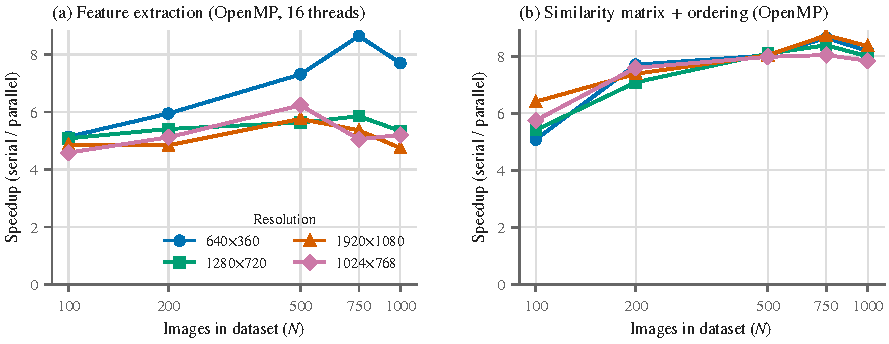
\includegraphics[width=0.96\textwidth]{figures/stage_speedup.pdf}
\caption{Speedup of the OpenMP stages (serial time divided by parallel time) as a function of dataset size, for each output resolution (means over $F\in\{10,20,30\}$).}
\label{fig:stagespeedup}
\end{figure*}

\begin{table}[t]
\caption{Mean speedup (S/P) by output resolution over all $N$ and $F$ (15 configurations each). ``Enc.\ \%'' is the blend+encode share of the serial pipeline time.}
\label{tab:speedup}
\centering
\footnotesize
\setlength{\tabcolsep}{4pt}
\begin{tabular}{@{}lccccc@{}}
\toprule
Resolution & Feat. & Sim.+ord. & Blend+enc. & Total & Enc.\ \% \\
\midrule
640$\times$360 & 6.95 & 7.53 & 1.04 & 1.09 & 95.3 \\
1280$\times$720 & 5.46 & 7.39 & 1.09 & 1.11 & 97.3 \\
1920$\times$1080 & 5.11 & 7.78 & 1.10 & 1.12 & 97.7 \\
1024$\times$768 & 5.24 & 7.44 & 1.08 & 1.11 & 97.2
\\
\bottomrule
\end{tabular}
\end{table}

\subsection{End-to-end results}
Fig.~\ref{fig:total} (a) plots the pipeline time against the number of frames written, on logarithmic axes: all resolutions follow straight lines of unit slope, and parallel runs lie just below serial runs. Fig.~\ref{fig:total} (b) shows that the end-to-end speedup is between $1.04\times$ and $1.15\times$ (mean $1.12\times$), almost independent of $N$ beyond $N{=}200$ and slightly lower at $640{\times}360$. Across the whole study, the serial runs total $1.00$\,h of pipeline time and the parallel runs $0.88$\,h. The longest single run ($N{=}1000$, $1920{\times}1080$, $F{=}30$, $30{,}970$ frames) took $337$\,s serially and $298$\,s in parallel.

\begin{figure*}[t]
\centering
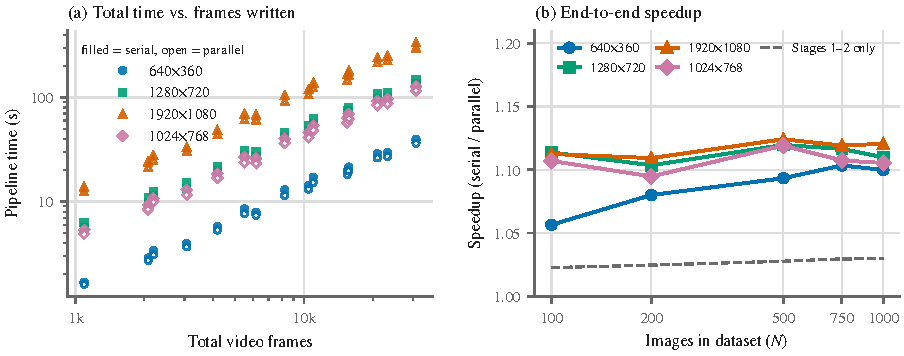
\includegraphics[width=0.96\textwidth]{figures/total_time_speedup.pdf}
\caption{(a) Pipeline time versus number of frames written (log--log). Filled markers: serial; open markers: parallel. (b) End-to-end speedup versus dataset size (means over $F$). The dashed line is the speedup that would result from accelerating only Stages~1--3 and leaving blend + encode at its serial time.}
\label{fig:total}
\end{figure*}

\subsection{Effect of transition length}
Table~\ref{tab:frames} varies $F$ for $N{=}500$ at $1280\times720$. Pipeline time grows linearly with the number of frames, and the speedup is the same for all three settings.

\begin{table}[t]
\caption{Effect of the number of intermediate frames $F$ ($N{=}500$, $1280\times720$). S/P: serial/parallel pipeline time.}
\label{tab:frames}
\centering
\footnotesize
\setlength{\tabcolsep}{4pt}
\begin{tabular}{@{}rrrrrr@{}}
\toprule
$F$ & Frames $T$ & S (ms) & P (ms) & Speedup & P enc.\ ms/frame \\
\midrule
10 & 5490 & 31{,}031 & 27{,}752 & 1.12 & 5.01 \\
20 & 10480 & 53{,}888 & 48{,}269 & 1.12 & 4.58 \\
30 & 15470 & 74{,}905 & 66{,}619 & 1.12 & 4.29
\\
\bottomrule
\end{tabular}
\end{table}

%=====================================================================
\section{Analysis}

\subsection{The parallel stages scale, but sub-linearly}
The OpenMP stages run $7.9\times$ (features) and $7.5\times$ (similarity) faster on 16 threads. Neither approaches the thread count. We do not have profiling data to attribute this precisely; plausible contributors are that the CPU has $6$ performance and $4$ efficiency cores rather than $16$ equal ones (so 16 threads are not 16 full cores), that decoding and resizing are memory-bandwidth-bound, and, for the similarity stage, that the triangular iteration space leaves some imbalance and that the stage is short (4--400\,ms serial) and therefore sensitive to start-up cost at small $N$. The latter is consistent with Fig.~\ref{fig:stagespeedup}(b), where the speedup rises with $N$ and then flattens near $8\times$. Section~\ref{sec:threads} later measures the scaling of these stages directly. Per image, feature extraction costs $1.07$\,ms (serial) versus $0.14$\,ms (parallel) at $640\times360$ and $7.2$\,ms versus $0.92$\,ms at $1920\times1080$. With the strict baseline the speedup no longer depends on the resolution, so the explanation we first suggested for a better scaling at low resolution (a larger fixed share of JPEG decoding, the source images being tiny) is not needed; the earlier dependence is consistent with OpenCV's thread pool helping the baseline more at high resolution, which we have not isolated further.

\subsection{Encoding dominates, which caps the end-to-end gain}
Blend and encode takes $91$--$98\%$ of the serial pipeline time (mean $95.9\%$), and $98.8$--$99.7\%$ of the parallel pipeline time (Fig.~\ref{fig:breakdown}; Table~\ref{tab:speedup}). Its cost is proportional to the number of frames (Fig.~\ref{fig:total}a; Table~\ref{tab:frames}) and grows with the frame area: for the parallel build the stage costs $1.3$\,ms per frame at $640{\times}360$, $4.0$ at $1024{\times}768$, $4.7$ at $1280{\times}720$ and $10.4$\,ms at $1920{\times}1080$. By Amdahl's law \cite{amdahl1967}, speeding up a fraction $p$ of the run time by a factor $s$ gives an overall speedup $1/\big((1-p)+p/s\big)$, bounded by $1/(1-p)$. Here Stages~1--3 make up only $p\approx 2$--$9\%$ of the serial time; accelerating them alone would give a speedup of $1.02$--$1.08\times$ (mean $1.04\times$, dashed line in Fig.~\ref{fig:total}b), however fast they became. This is the same structure that Fan \emph{et al.}\ exploit in the opposite direction: they identify the dominant stage of their pipeline and redesign around it \cite{fan2024}; in our pipeline the dominant stage is video encoding, not feature analysis.

\subsection{GPU blending gives a small additional gain}
The observed mean end-to-end speedup, $1.12\times$, is larger than the $1.04\times$ explained by Stages~1--3, because the blend-and-encode stage itself is $1.08\times$ faster on average ($0.99$--$1.13\times$) when the blend runs on the GPU. At $1920\times1080$ it falls from $11.4$ to $10.4$\,ms per frame, i.e.\ the GPU saves about $1$\,ms per frame net of the $\approx 6$\,MB device-to-host copy that each frame requires. This is an inference from the totals; we did not time blending separately. It shows that the per-pixel blend is cheap even on the CPU compared with encoding a frame, so offloading it cannot change the picture by more than about $10\%$. The GPU gain is smallest at $640\times360$, where the blend work per frame is smallest and the fixed per-frame launch and transfer overheads are largest.

\subsection{Longer transitions are slightly cheaper per frame}
Table~\ref{tab:frames} shows the encode cost per frame falling from $5.0$ to $4.6$ to $4.3$\,ms as $F$ increases from $10$ to $30$, while total time remains proportional to $T$. Consecutive blended frames differ only slightly, and an inter-frame video codec compresses such frames well, whereas the first frame of each pair is a new image; we did not verify this with codec statistics.

\subsection{Threats to validity}
Each configuration was run once, so run-to-run variance is not quantified; the smoothness of the curves (Figs.~\ref{fig:stagespeedup} and~\ref{fig:total}) suggests it is small compared with the effects discussed, but the individual stage numbers for the shortest stages should be read with care. The serial baseline of the final results was re-measured in a separate sweep with OpenCV's thread pool disabled, whereas the parallel builds were measured with the pool at its default (Section~\ref{sec:threads}). All results come from one laptop whose clocks may vary with temperature, and from one codec (\texttt{mp4v}) selected through OpenCV; a hardware encoder or a multi-threaded encoder would change the balance between stages. We did not measure ordering quality or interpolation quality (e.g.\ PSNR), and the cross-dissolve does not model motion, so these results speak to execution time only.

%=====================================================================
\section{Overlapping Blending and Encoding with a Producer--Consumer Queue}
\label{sec:queue}
The analysis above shows that blend + encode dominates, and that in the first parallel build the two halves of that stage run one after the other: for every frame the host launches the kernel, waits for it (the wrapper synchronises), copies the frame back and only then hands it to the encoder, so the encoder is idle while the GPU works and vice versa. This section implements the second future-work direction of the first version of this study: overlapping blending with encoding through a producer--consumer queue and CUDA streams \cite{dijkstra1965,nvidia_cudaguide}. We refer to the original parallel build as \emph{P$_1$} (synchronous) and to the new one as \emph{P$_2$} (queue). The serial baseline and all stages other than blend + encode are unchanged.

\subsection{Design}
Fig.~\ref{fig:queue} shows the structure. The main thread is the \emph{producer}: for each image pair it uploads the two images to the device and, for each intermediate frame, takes a free \emph{slot}, launches the blend kernel on that slot's CUDA stream and enqueues an asynchronous device-to-host copy into the slot's page-locked (pinned) host buffer, without waiting for it. It then appends the slot to a FIFO \emph{ready queue}. A second thread, the \emph{consumer}, pops items in order, synchronises with the stream of the slot it received, writes the frame to the \texttt{VideoWriter} and returns the slot to the free pool. The original images themselves (the first frame of each pair and the last image) are queued as direct items that need no GPU work, which keeps the output order identical to Eq.~\eqref{eq:frames}.

\begin{figure}[t]
\centering
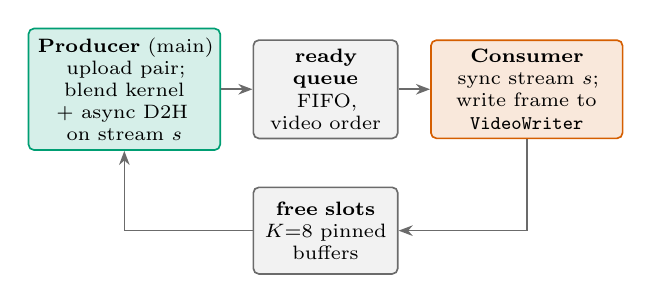
\begin{tikzpicture}[
  node distance=4mm,
  b/.style={draw, rounded corners=2pt, minimum height=11mm, text width=22mm, align=center, font=\scriptsize, line width=0.6pt},
  gp/.style={b, fill=cGreen!16, draw=cGreen},
  sq/.style={b, fill=cOrange!14, draw=cOrange},
  qq/.style={b, fill=black!5, draw=cGrey, text width=16mm},
  arr/.style={-{Stealth[length=1.8mm]}, line width=0.6pt, draw=cGrey}
]
\node[gp] (prod) {\textbf{Producer} (main)\\ upload pair; blend kernel\\+ async D2H on stream $s$};
\node[qq, right=4mm of prod] (rq) {\textbf{ready queue}\\FIFO, video order};
\node[sq, right=4mm of rq] (cons) {\textbf{Consumer}\\ sync stream $s$;\\ write frame to\\ \texttt{VideoWriter}};
\node[qq, below=6mm of rq] (fq) {\textbf{free slots}\\$K{=}8$ pinned buffers};
\draw[arr] (prod) -- (rq);
\draw[arr] (rq) -- (cons);
\draw[arr] (cons.south) |- (fq.east);
\draw[arr] (fq.west) -| (prod.south);
\end{tikzpicture}
\caption{Producer--consumer structure of the queue build. The producer blocks when no free slot is available, which bounds the number of frames in flight; the consumer returns a slot only after the frame has been written.}
\label{fig:queue}
\end{figure}

Three details matter for correctness. (a)~\emph{Back-pressure.} A fixed pool of $K{=}8$ slots, each owning one output buffer on the device, one pinned host buffer and one stream, bounds the memory in flight; because slots are reused only after the consumer has written them, no frame is overwritten before it is encoded. (b)~\emph{Image buffers.} The device holds two image-pair buffers used alternately for consecutive pairs; before a buffer is overwritten, events recorded on every slot stream guarantee that the kernels of the pair that last used it have finished. (c)~\emph{Errors.} Any CUDA error closes both queues, which unblocks the other thread, and the program exits with an error instead of hanging. The kernel wrapper was changed to take a stream, to return the launch status, and to drop its per-launch \texttt{cudaDeviceSynchronize}. With this structure the CPU-side encode of frame $t$ overlaps with the GPU blend and copy of frames $t{+}1,\dots,t{+}K$, so the per-frame time can approach the larger of the two rather than their sum.

\subsection{Experiment}
We re-ran only the parallel executable over the same grid as before ($5$ datasets $\times$ $4$ resolutions $\times$ $3$ values of $F$ $=60$ runs, $50$\,min $44$\,s in total), on the same machine and software, with the same driver (extended with a flag that selects the serial, the parallel or both executables). The P$_1$ numbers are those of the first sweep, and the serial baseline is the strictly single-threaded re-run described in Section~\ref{sec:threads}; comparisons between P$_2$, P$_1$ and serial therefore span three sweeps (P$_1$ ran from 17:46 to 19:40 and P$_2$ from 22:06 to 22:57 on 27 October, about two and a half hours apart, and the serial re-run from 00:19 to 01:19 the following night; Section~\ref{sec:queue-validity}). As an output check, on \texttt{landscape\_100} at $1280\times720$ and $F{=}20$ both the serial build and P$_2$ produced $2080$ frames, and after decoding their frames differ by a mean absolute value of $0.31$ intensity levels (largest per-frame mean $1.35$), i.e.\ codec noise, as in the earlier check. A run with $F{=}0$, which has no blend work, also completes correctly.

\subsection{Results}
All $60$ runs completed. P$_2$ is faster than P$_1$ in \emph{every} configuration: the end-to-end gain over P$_1$ is $1.01$--$1.15\times$ (mean $1.07\times$), and the gain over the serial build rises from $1.04$--$1.15\times$ (mean $1.12\times$) to $1.14$--$1.25\times$ (mean $1.19\times$). Summed over the grid, the pipeline time of the $60$ configurations is $1.00$\,h serially, $0.88$\,h with P$_1$ and $0.84$\,h with P$_2$; the longest run ($N{=}1000$, $1920\times1080$, $F{=}30$, $30{,}970$ frames) took $337$\,s, $298$\,s and $276$\,s respectively. Table~\ref{tab:queue-main} gives the $1920\times1080$, $F{=}20$ slice corresponding to Table~\ref{tab:main}, and Table~\ref{tab:queue-res} summarises the effect by resolution.

\begin{table}[t]
\caption{Pipeline time (ms) at $1920\times1080$, $F{=}20$: serial (S), synchronous parallel (P$_1$) and queue-based parallel (P$_2$), with speedups over S.}
\label{tab:queue-main}
\centering
\footnotesize
\setlength{\tabcolsep}{3.2pt}
\begin{tabular}{@{}rrrrrr@{}}
\toprule
$N$ & S & P$_1$ & P$_2$ & S/P$_1$ & S/P$_2$ \\
\midrule
100 & 24{,}413 & 21{,}465 & 19{,}994 & 1.14 & 1.22 \\
200 & 48{,}677 & 43{,}799 & 40{,}138 & 1.11 & 1.21 \\
500 & 121{,}689 & 107{,}156 & 99{,}514 & 1.14 & 1.22 \\
750 & 182{,}916 & 162{,}743 & 154{,}470 & 1.12 & 1.18 \\
1000 & 243{,}663 & 214{,}828 & 198{,}840 & 1.13 & 1.23
\\
\bottomrule
\end{tabular}
\end{table}

\begin{table}[t]
\caption{Effect of the queue by output resolution (means over all $N$ and $F$, $15$ configurations each). ``Enc.'' is the blend + encode time per frame (ms).}
\label{tab:queue-res}
\centering
\footnotesize
\setlength{\tabcolsep}{3.2pt}
\begin{tabular}{@{}lccccc@{}}
\toprule
Resolution & Enc.\ P$_1$ & Enc.\ P$_2$ & S/P$_1$ & P$_1$/P$_2$ & S/P$_2$ \\
\midrule
$640{\times}360$ & 1.28 & 1.15 & 1.08 & 1.11 & 1.20 \\
$1280{\times}720$ & 4.68 & 4.51 & 1.13 & 1.04 & 1.17 \\
$1920{\times}1080$ & 10.37 & 9.70 & 1.13 & 1.07 & 1.21 \\
$1024{\times}768$ & 4.03 & 3.85 & 1.12 & 1.05 & 1.17
\\
\bottomrule
\end{tabular}
\end{table}

The gain is largest at $640\times360$ ($1.11\times$ over P$_1$; $1.28\to1.15$\,ms per frame) and at $1920\times1080$ ($1.07\times$; $10.4\to9.7$\,ms), and smallest at $1280\times720$ ($1.04\times$). At the smallest resolution the fixed per-frame costs of P$_1$---a synchronising launch and a copy per frame---are the largest share of the work, which is what the queue removes. At $1920\times1080$ the saving of about $0.7$\,ms per frame is of the size expected from hiding a $\approx 6$\,MB device-to-host copy and the blend behind the encoder. Both readings are inferences from the totals; we did not time the encoder or the GPU work in isolation.

\subsection{What still limits the pipeline}
The gain is small because the queue can hide the GPU work only up to the time the encoder takes, and the encoder is the bulk of that time: in P$_2$, blend + encode is still $98.8$--$99.7\%$ of the pipeline time (mean $99.4\%$). We checked this directly by sampling the running P$_2$ process in the middle of the sweep (a single sample at $1024\times768$, so indicative rather than a systematic profile): the GPU showed $6\%$ utilisation and $1\%$ memory-bandwidth utilisation, and per-thread CPU usage showed one thread at about $95\%$ while the other fifteen were idle. That busy thread is the consumer running the \texttt{mp4v} encoder; the producer spends its time blocked on free slots, so the GPU is idle most of the time. The device memory in use ($\approx 180$\,MiB of $6$\,GiB) is small because only twelve frame-sized buffers (four image buffers and eight output buffers) and the CUDA context live on the GPU, while the resized images stay in host memory; it is not a resource that limits the speed.

This has a direct consequence for the future-work options. Giving the GPU more work, or more threads or streams, cannot help, because the producer is already waiting for the consumer. What helps is more \emph{encoders}: the sixteen idle CPU threads can be used by writing independent video segments in parallel and concatenating them without re-encoding, and the encoding itself can be moved off the CPU with a hardware encoder. We expect the former to give the larger share of its gain on the CPU side (bounded by the six performance and four efficiency cores and by memory bandwidth) while keeping the codec unchanged, so that comparisons with the serial build remain like for like; a hardware encoder would change the codec and needs its own comparison. Section~\ref{sec:segments} implements and evaluates the former.

\subsection{Threats to validity}
\label{sec:queue-validity}
P$_1$, P$_2$ and the serial baseline come from three separate sweeps on the same laptop (P$_2$ started about two and a half hours after the P$_1$ sweep had finished, and the serial re-run about an hour and a half after P$_2$ ended); temperature, background load and clock behaviour may differ between them, so the speedups over serial carry an uncertainty that the P$_2$/P$_1$ comparison shares. That P$_2$ is faster in all $60$ configurations supports the direction of the effect but not its exact size. Each configuration was again run once. The utilisation figures are a single mid-run sample, and the explanation of the per-resolution differences is not verified by separate timing. As before, the results concern execution time only, with output equivalence checked on a single configuration.

%=====================================================================
\section{Parallel Video Segments}
\label{sec:segments}
Section~\ref{sec:queue} showed that after the GPU work is hidden, one encoder thread is the limit while fifteen CPU threads and most of the GPU are idle. This section makes the encoder itself parallel by writing independent video segments concurrently and joining them without re-encoding (future-work direction~(iii) of the first version). We call the resulting build \emph{P$_3$}.

\subsection{Design}
The ordered image sequence has $N{-}1$ image pairs. For a number of segments $K$, segment $j$ receives the contiguous range of pairs $\lfloor j(N{-}1)/K\rfloor,\dots,\lfloor (j{+}1)(N{-}1)/K\rfloor-1$, and the last segment additionally receives the final image, so the $K$ segments together contain exactly the $T$ frames of Eq.~\eqref{eq:frames}. Every segment runs the complete queue structure of Section~\ref{sec:queue} (Fig.~\ref{fig:queue}) independently: its own producer, encoder thread, \texttt{VideoWriter}, slot pool, CUDA streams and device buffers, writing its own temporary file. When all segments are done the files are joined by FFmpeg's concat demuxer in stream-copy mode \cite{ffmpeg_concat} (\texttt{-c copy}), which does not decode or re-encode, and the temporary files are deleted. $K{=}1$ writes one file directly, needs no FFmpeg and is identical to P$_2$. The segment count is a command-line option (\texttt{--segments}); the timed ``blend + encode'' stage includes the join. Device and pinned memory grow linearly with $K$ ($\approx 1.0$\,GiB of GPU memory at $K{=}12$ and $1920\times1080$, including the CUDA context), whereas the resized images are shared by all segments.

\subsection{Choosing $K$}
We chose $K$ with a pilot on \texttt{landscape\_100} at $1280\times720$ and $F{=}20$ ($2080$ frames), running each $K$ three times, interleaved to avoid favouring one value through thermal drift, and taking the median (Table~\ref{tab:pilot}, Fig.~\ref{fig:master}c). The time falls almost linearly up to $K{=}2$ (efficiency $0.94$ relative to $K{=}1$), then flattens: $K{=}8$ gives $4.9\times$, $K{=}12$ gives $5.2\times$, and $K{=}16$ is no faster than $K{=}12$. We used $K{=}12$ for the full sweep. The choice rests on this one setting.

\begin{table}[t]
\caption{Segment-count pilot (\texttt{landscape\_100}, $1280\times720$, $F{=}20$; median of three runs). Speedup and efficiency are relative to $K{=}1$, which equals P$_2$.}
\label{tab:pilot}
\centering
\footnotesize
\setlength{\tabcolsep}{5pt}
\begin{tabular}{@{}rrrr@{}}
\toprule
$K$ & Blend + encode (s) & Speedup & Efficiency \\
\midrule
1 & 9.62 & 1.00 & 1.00 \\
2 & 5.11 & 1.88 & 0.94 \\
4 & 2.88 & 3.34 & 0.83 \\
6 & 2.22 & 4.33 & 0.72 \\
8 & 1.98 & 4.87 & 0.61 \\
12 & 1.84 & 5.24 & 0.44 \\
16 & 1.84 & 5.24 & 0.33
\\
\bottomrule
\end{tabular}
\end{table}

\subsection{Experiment and output check}
With $K{=}12$ we re-ran only the parallel executable over the same $60$-configuration grid (the sweep took $9$\,min $29$\,s, against $50$\,min $44$\,s for P$_2$), starting about eleven minutes after the P$_2$ sweep had finished, on the same hardware and software, with FFmpeg~9.0.2 for the join. P$_1$ is again taken from the first sweep and the serial baseline from the strictly single-threaded re-run. As an output check, on \texttt{landscape\_100} at $1280\times720$ and $F{=}20$ the $K{=}4$ and $K{=}12$ videos both have $2080$ frames, and after decoding they differ from the serial video by a mean absolute value of $0.91$ and $1.13$ intensity levels (largest per-frame mean $2.4$ and $2.6$). This is larger than the $0.31$ of P$_2$, plausibly because every segment restarts the encoder's rate control, but it is still at codec-noise level and shows no boundary artefact. We did not measure file sizes.

\subsection{Results}
All $60$ runs completed. Over the whole grid P$_3$ is $5.3\times$ faster than P$_2$ on average (per-configuration range $0.61$--$5.88\times$) and $5.6\times$ faster than P$_1$; against the serial build the mean per-configuration speedup is $6.3\times$ ($0.74$--$7.16\times$), and the ratio of total times is $6.55\times$. The pipeline times of the $60$ configurations sum to $1.00$\,h (serial), $0.88$\,h (P$_1$), $0.84$\,h (P$_2$) and $0.15$\,h (P$_3$). The longest run ($N{=}1000$, $1920\times1080$, $F{=}30$, $30{,}970$ frames) took $337$\,s, $298$\,s, $276$\,s and $50$\,s respectively. Table~\ref{tab:seg-main} gives the $1920\times1080$, $F{=}20$ slice, and Table~\ref{tab:seg-res} the effect by resolution: the blend + encode cost per frame at $1920\times1080$ falls from $9.7$ to $1.7$\,ms.

\begin{table}[t]
\caption{Pipeline time (ms) at $1920\times1080$, $F{=}20$ for P$_2$ and P$_3$, and speedups of P$_3$ over P$_2$ and over serial (S).}
\label{tab:seg-main}
\centering
\footnotesize
\setlength{\tabcolsep}{5pt}
\begin{tabular}{@{}rrrrr@{}}
\toprule
$N$ & P$_2$ & P$_3$ & P$_2$/P$_3$ & S/P$_3$ \\
\midrule
100 & 19{,}994 & 3{,}631 & 5.51 & 6.72 \\
200 & 40{,}138 & 6{,}825 & 5.88 & 7.13 \\
500 & 99{,}514 & 17{,}862 & 5.57 & 6.81 \\
750 & 154{,}470 & 26{,}515 & 5.83 & 6.90 \\
1000 & 198{,}840 & 35{,}225 & 5.64 & 6.92
\\
\bottomrule
\end{tabular}
\end{table}

\begin{table}[t]
\caption{Effect of the segments by output resolution (means over all $N$ and $F$). ``Enc.'' is the blend + encode time per frame (ms).}
\label{tab:seg-res}
\centering
\footnotesize
\setlength{\tabcolsep}{5pt}
\begin{tabular}{@{}lcccc@{}}
\toprule
Resolution & Enc.\ P$_2$ & Enc.\ P$_3$ & P$_2$/P$_3$ & S/P$_3$ \\
\midrule
$640{\times}360$ & 1.15 & 0.34 & 4.87 & 5.85 \\
$1280{\times}720$ & 4.51 & 0.82 & 5.34 & 6.23 \\
$1920{\times}1080$ & 9.70 & 1.67 & 5.64 & 6.84 \\
$1024{\times}768$ & 3.85 & 0.72 & 5.20 & 6.09
\\
\bottomrule
\end{tabular}
\end{table}

The speedup is nearly independent of problem size: the ratio of total serial to P$_3$ time is $6.6$, $6.6$, $6.6$ and $6.5$ for $N{=}200$, $500$, $750$ and $1000$, and lower ($5.6$) only for $N{=}100$; by transition length it is $6.4$, $6.6$ and $6.6$ for $F{=}10$, $20$ and $30$. The one configuration slower than the serial build is the first and smallest of the sweep ($N{=}100$, $640\times360$, $F{=}10$, $1090$ frames: $2.27$\,s against $1.68$\,s serial and $1.39$\,s for P$_2$). For such a short job the fixed costs of twelve buffer sets, twelve writers and the join are a large share; we did not isolate which, nor whether the first position in the sweep contributed. Excluding it, the per-configuration speedup over serial is $4.7$--$7.2\times$ (mean $6.3\times$).

The OpenMP stages, re-measured in this sweep, are consistent with the earlier ones (feature extraction $7.2\times$ mean, $5.9$--$8.4\times$, against $7.9\times$ for P$_1$; similarity and ordering $7.0\times$ against $7.5\times$). They matter more now: feature extraction is $3.2\%$ of the P$_3$ pipeline time on average (up to $6.1\%$), the sequential ordering $0.3\%$ (up to $2.2\%$), and blend + encode $96.5\%$ (mean; $91.8$--$99.2\%$).

\subsection{What limits P$_3$}
In a single mid-run sample of P$_3$ ($N{=}1000$, $1920\times1080$, $F{=}20$, $K{=}12$) the GPU showed $38\%$ utilisation (against $6\%$ for P$_2$), $9\%$ memory-bandwidth utilisation and $1010$\,MiB in use, and the CPU was about $84\%$ busy overall. The sample is indicative only. Together with the flat pilot curve beyond $K{=}12$, it suggests that the encoders now fill the CPU: the machine has six performance and four efficiency cores, and encoder threads beyond that number cannot add throughput. The remaining headroom is therefore on the GPU (still mostly idle) rather than on the CPU, which points to hardware encoding as the next step. Section~\ref{sec:threads} tests the claim about the encoders with independent concurrent encodes.

\subsection{Threats to validity}
The $K$ pilot covers one dataset and one setting, and a different $K$ may be better for other sizes (the small-job slowdown suggests that $K$ should depend on the number of frames). The sweeps for serial/P$_1$, P$_2$ and P$_3$ are separate runs on one laptop, so ratios across sweeps share the uncertainty discussed in Section~\ref{sec:queue-validity}; each configuration was run once. The utilisation figures are single samples. Segment boundaries were checked only through decoded-frame differences on one configuration.

%=====================================================================
\section{Master Comparison of the Builds}
\label{sec:master}
We now compare the builds: the strictly single-threaded serial baseline (S), the synchronous OpenMP/CUDA build (P$_1$), the queue build (P$_2$), the segmented build (P$_3$, $K{=}12$, $16$ threads) and a variant of P$_3$ restricted to six threads (six OpenMP threads and six segments), over the same $60$ configurations. Totals and ratios below are computed over all $60$ configurations ($\psi=\sum T_S/\sum T_P$), and ``mean'' refers to the mean of per-configuration ratios.

\subsection{Performance summary}
Table~\ref{tab:master-perf} and Fig.~\ref{fig:master} summarise the builds. Each step improves on the previous one, but by very different amounts: the two steps that overlap or parallelise the \emph{already parallel} parts (P$_1$, P$_2$) bring $1.13\times$ and $1.19\times$ over serial, while parallelising the encoder (P$_3$) brings $6.55\times$ (and $5.3\times$ with only six threads, Section~\ref{sec:final}).

\begin{table}[t]
\caption{Summary over the $60$ configurations. $T$: total pipeline time; $\psi$: ratio of total times; range: per-configuration speedup over serial; Longest: the $N{=}1000$, $1920{\times}1080$, $F{=}30$ run; Enc.: blend + encode ms per frame at $1920{\times}1080$.}
\label{tab:master-perf}
\centering
\footnotesize
\setlength{\tabcolsep}{3pt}
\begin{tabular}{@{}lrrcrr@{}}
\toprule
Build & $T$ (h) & $\psi$ & Range & Longest (s) & Enc. \\
\midrule
Serial & 1.00 & 1.00 & 1.00--1.00 & 337 & 11.40 \\
P$_1$ sync & 0.88 & 1.13 & 1.04--1.15 & 298 & 10.37 \\
P$_2$ queue & 0.84 & 1.19 & 1.14--1.25 & 276 & 9.70 \\
P$_3$ segments & 0.15 & 6.55 & 0.74--7.16 & 50 & 1.67 \\
P$_3$, 6 threads & 0.19 & 5.29 & 2.88--5.89 & 59 & 2.08
\\
\bottomrule
\end{tabular}
\end{table}

\begin{figure*}[t]
\centering
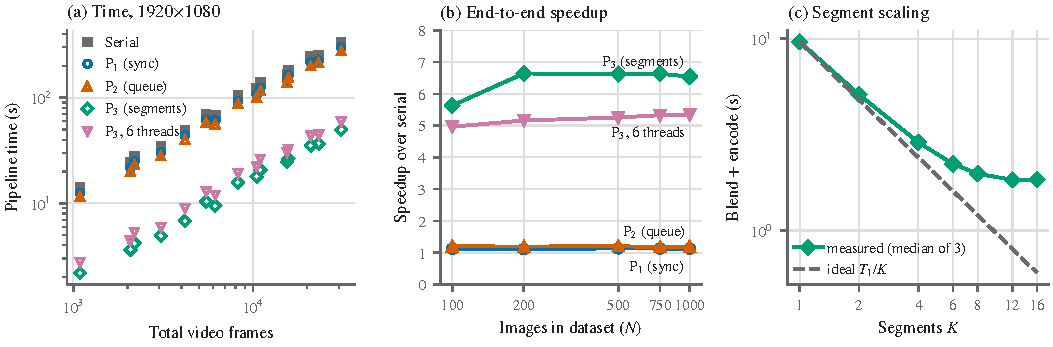
\includegraphics[width=0.96\textwidth]{figures/master_comparison.pdf}
\caption{Master comparison. (a)~Pipeline time versus frames written at $1920\times1080$ for all builds (log--log; each marker is one $N$, $F$ combination). (b)~Speedup over serial versus dataset size (ratio of total times over resolutions and $F$). (c)~Blend + encode time versus the number of segments $K$ in the pilot, with the ideal $T_1/K$ line.}
\label{fig:master}
\end{figure*}

\subsection{Speedup, efficiency and cost}
For a run on $p$ processing elements with time $T_p$ against the best serial time $T_s$, the classical quantities are the speedup $\psi=T_s/T_p$, the efficiency $E=\psi/p$ and the cost $C=p\,T_p$; a parallel system is \emph{cost-optimal} if its cost grows as fast as the serial time, $C=\Theta(T_s)$, i.e.\ if its efficiency is bounded below by a constant \cite{grama2003}. We take $p=16$, the hardware threads of the OpenMP team, for P$_1$--P$_3$ and $p=6$ for the six-thread variant, and report the efficiency against the physical cores as a sensitivity check; the GPU and the FFmpeg join are not counted as processors, which flatters all parallel builds, so the figures are optimistic. Table~\ref{tab:master-metrics} gives the results.

\begin{table}[t]
\caption{Classical metrics against the serial build over the $60$ configurations. $p$: threads used; $E_p=\psi/p$; $E_c=\psi/\min(p,10)$, the efficiency against the physical cores used; Cost: $pT_p/T_s$ (cost-optimal $\approx 1$); $e$: Karp--Flatt experimentally determined serial fraction for this $p$; $1/e$: the corresponding Amdahl bound.}
\label{tab:master-metrics}
\centering
\footnotesize
\setlength{\tabcolsep}{3pt}
\begin{tabular}{@{}lrrrrrrr@{}}
\toprule
Build & $p$ & $\psi$ & $E_p$ & $E_c$ & Cost & $e$ & $1/e$ \\
\midrule
P$_1$ sync & 16 & 1.13 & 0.070 & 0.113 & 14.2 & 0.879 & 1.1 \\
P$_2$ queue & 16 & 1.19 & 0.074 & 0.119 & 13.4 & 0.829 & 1.2 \\
P$_3$ segments & 16 & 6.55 & 0.409 & 0.655 & 2.4 & 0.096 & 10.4 \\
P$_3$, 6 threads & 6 & 5.29 & 0.882 & 0.882 & 1.1 & 0.027 & 37.3
\\
\bottomrule
\end{tabular}
\end{table}

None of the 16-thread builds is cost-optimal. P$_1$ and P$_2$ spend $14.2\times$ and $13.4\times$ the serial cost ($14.2$ and $13.4$ thread-hours against $1.00$) for a $1.1$--$1.2\times$ speedup: with an efficiency of $0.07$, more than $90\%$ of the CPU capacity they claim is idle, in line with the one busy encoder thread seen in Section~\ref{sec:queue}. P$_3$ costs $2.4\times$ the serial run ($2.4$ thread-hours), $5.5\times$ less than P$_2$, with $E_{16}=0.41$ and $E_{10}=0.65$; with $p=10$ its cost would be $1.5\times$ serial. Of the 16-thread builds it is the closest, but it is not there; restricting the pipeline to six threads (Section~\ref{sec:final}) brings the cost to $1.13\times$ serial. Counting the GPU as a processing element would increase all costs.

\emph{Algorithm or hardware?} The causes differ between the builds. For P$_1$ and P$_2$ the cause is the \emph{software structure}: one sequential encoder performs about $99\%$ of the work, so the implied serial fraction is $0.83$--$0.88$ and the efficiency is capped near $1/(p\,e)\approx0.07$ for any hardware. For P$_3$ the algorithm's own serial part is negligible (the ordering takes $0.3\%$ of the time), so the shortfall comes from three sources, which Section~\ref{sec:threads} helps to separate. (a)~\emph{What $p$ counts.} The CPU has $10$ physical cores ($6$ performance cores with two hardware threads each and $4$ efficiency cores), so $16$ threads are not $16$ equal processors; against the $10$ cores the efficiency is $0.65$ rather than $0.41$. (b)~\emph{Hardware sharing}: the efficiency cores are slower, the cores share caches, memory bandwidth and power and thermal limits, and the pilot (Table~\ref{tab:pilot}) already shows an efficiency of $0.72$ at $K{=}6$ and a flat curve once the CPU is about $84\%$ busy. (c)~\emph{Our own overheads}: twelve buffer sets and writers, thread start-up and the FFmpeg join (Section~\ref{sec:threads} bounds these at a few percent). Finally, the criterion itself is strict: even well-tuned codes seldom keep an efficiency near $1$ on hyper-threaded, heterogeneous CPUs.

\emph{Could more hardware make it cost-optimal?} Not by adding more of the same. Cost-optimality requires the efficiency to stay bounded below as $p$ grows, but with a Karp--Flatt serial fraction $e$ that does not change with $p$ the speedup is $\psi(p)=1/\big(e+(1-e)/p\big)$ and the efficiency is $E(p)=1/\big(1+e(p-1)\big)$, which tends to $1/(e\,p)$: it \emph{falls} as processors are added, and the speedup is bounded by $1/e$ ($10.4$ for P$_3$). Requiring $E\ge c$ gives $p\le 1+(1/c-1)/e$. For $c=0.5$ this is $p\le 2.1$ for P$_1$ and $2.2$ for P$_2$---essentially one producer and one encoder, so these builds cannot usefully employ a third processor---and $p\le 11$ for P$_3$ (up to about $18$ if the smaller $e$ computed for $p=10$ is used), which is about the size of this machine. P$_3$ is therefore well matched to the laptop, and on a larger machine of the same kind its efficiency would drop. To reach $E=0.8$ at $p=16$ the serial fraction would have to fall to $e\le 0.017$ ($\psi\ge12.8$), about six times lower than measured. Because $e$ is flat in $N$ (Section~\ref{sec:master}D) it is overhead proportional to the work and is not amortised by larger inputs; reducing it needs lower per-frame overhead or more uniform hardware (full cores with more memory bandwidth per core), not simply more cores. The six-thread variant of Section~\ref{sec:final} agrees with this picture: with $p=6<1/e$ its efficiency is $0.88$. This model extrapolates from a single $p$, and the segment pilot shows that $e$ itself varies with $K$, so the figures are indications of scale, not predictions. The scaling studies of Section~\ref{sec:threads} show that the machine itself caps a CPU-bound OpenMP stage at about $8.4\times$ ($E_{16}\approx0.53$, $E_{10}\approx0.84$) and independent concurrent encodes at $7.2\times$ on $16$ copies, and that P$_3$'s blend + encode reaches $94\%$ ($12$ segments) and $98\%$ (six threads) of the independent-encode speedup at the same thread count ($1280\times720$), so the hardware accounts for most of the shortfall in efficiency and our own overhead for only a few percent.

\subsection{Amdahl and Karp--Flatt}
Amdahl's law \cite{amdahl1967} bounds the speedup by $1/(1-p_\parallel)$, where $p_\parallel$ is the parallelisable fraction. The Karp--Flatt metric \cite{karpflatt1990} inverts it: from a measured $\psi$ on $p$ processors, $e=(1/\psi-1/p)/(1-1/p)$ is the serial fraction \emph{implied} by the measurement, and $1/e$ is the corresponding bound. For P$_1$ and P$_2$ it gives $e=0.88$ and $0.83$, i.e.\ bounds of only $1.14\times$ and $1.21\times$: the builds behave as if $83$--$88\%$ of their time were serial, which is of the same order as the encoder's $99.4\%$ share of their pipeline time. For P$_3$, $e$ falls to $0.096$ (bound $10.4\times$ at the same overhead). Across dataset sizes $e$ is stable, $0.094$--$0.096$ for $N\ge 200$ and $0.123$ for $N{=}100$, which says that the shortfall behaves like a constant fraction rather than growing with $N$; the larger value at $N{=}100$ is consistent with start-up overheads weighing more in short runs. $e$ lumps together true serial work and parallel overhead and cannot separate them: for P$_3$ the sequential ordering stage is only $0.3\%$ of the time, so most of the $0.096$ must be overhead or imperfect scaling of the parallel stages (heterogeneous cores, memory bandwidth, thread start-up, the join); Section~\ref{sec:threads} separates them by measuring independent encodes, and finds that the pipeline's own share is small.

\subsection{Scalability and Gustafson's view}
\emph{Strong scaling} in the number of segments (Table~\ref{tab:pilot}, Fig.~\ref{fig:master}c) is good at small $K$ and saturates: efficiency relative to $K{=}1$ is $0.94$, $0.83$ and $0.61$ for $K{=}2$, $4$ and $8$, and $0.44$ at $K{=}12$, with no gain from $K{=}12$ to $16$; on this machine the encoders run out of cores. (Independent encodes still gain a little between $12$ and $16$ copies, $6.7\to7.2\times$, so part of the flat pilot curve is probably fixed cost in this short job of about $1.8$\,s; we did not isolate it.) \emph{Scaling with problem size} is where Gustafson's view \cite{gustafson1988} applies: with a serial fraction $\alpha$ of the parallel run time, the scaled speedup is $p-\alpha(p-1)$. The only stage that is not parallelised in P$_3$, the ordering, takes $\alpha\approx0.003$ of the time, which would predict a scaled speedup near $15.9$; the measured $6.55$ shows again that the limit is not a serial fraction but the efficiency of the parallel stages. The same data speak to \emph{isoefficiency} \cite{grama2003}: the efficiency of P$_3$ stays at $0.41$--$0.42$ for $N$ from $200$ to $1000$ and across $F$ ($0.40$--$0.41$), so no growth of the problem is needed to hold the efficiency once the job is not tiny, whereas for $N{=}100$ it is lower ($0.35$) because of fixed costs. The efficiency is bounded by the machine, not by the problem size.

\subsection{Thread and encoder scaling: a hardware ceiling}
\label{sec:threads}
To judge how much of P$_3$'s shortfall is the machine, we need a reference for what this CPU can deliver at all. We therefore measured the OpenMP stages with an explicit thread count (a new \texttt{--threads} option; \texttt{--cv-threads} sets the size of OpenCV's own pool, see below) for $t\in\{1,2,4,6,8,10,12,16\}$, on $N\in\{500,1000\}$ at $1280\times720$ and $1920\times1080$ with $F{=}0$ and $12$ segments (only the analysis-stage times are used; the short encode does not affect them), three interleaved repetitions each, taking medians. OpenCV's pool was set to one thread so that OpenMP is the only parallelism in these stages, and the baseline is the serial build with the same setting, i.e.\ strictly single-threaded. Table~\ref{tab:threads} and Fig.~\ref{fig:threads} give the means over the four configurations.

\begin{table}[t]
\caption{OpenMP scaling of the two analysis stages (means over $N\in\{500,1000\}$ and $1280{\times}720$, $1920{\times}1080$). $\psi$: speedup over the strictly single-threaded serial build; $E=\psi/t$; $e$: Karp--Flatt serial fraction. F: feature extraction; S: similarity + ordering.}
\label{tab:threads}
\centering
\footnotesize
\setlength{\tabcolsep}{3.5pt}
\begin{tabular}{@{}rrrrrrr@{}}
\toprule
$t$ & $\psi_F$ & $E_F$ & $e_F$ & $\psi_S$ & $E_S$ & $e_S$ \\
\midrule
1 & 1.00 & 1.00 & 0.000 & 1.00 & 1.00 & 0.000 \\
2 & 1.99 & 0.99 & 0.006 & 1.95 & 0.98 & 0.023 \\
4 & 3.86 & 0.96 & 0.012 & 3.81 & 0.95 & 0.016 \\
6 & 5.42 & 0.90 & 0.021 & 5.53 & 0.92 & 0.017 \\
8 & 6.15 & 0.77 & 0.043 & 6.41 & 0.80 & 0.036 \\
10 & 7.10 & 0.71 & 0.045 & 7.89 & 0.79 & 0.030 \\
12 & 7.52 & 0.63 & 0.054 & 8.04 & 0.67 & 0.045 \\
16 & 8.43 & 0.53 & 0.060 & 8.22 & 0.51 & 0.063
\\
\bottomrule
\end{tabular}
\end{table}

\begin{figure*}[t]
\centering
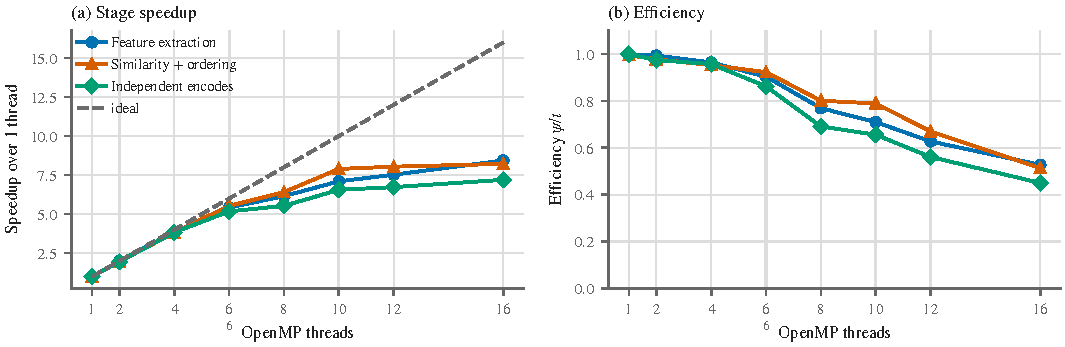
\includegraphics[width=0.72\textwidth]{figures/thread_scaling.pdf}
\caption{(a) Speedup and (b) efficiency of the OpenMP stages versus the number of threads, and of independent concurrent encodes versus the number of copies (relative to one copy). Vertical lines mark the $6$ performance cores and the $10$ physical cores.}
\label{fig:threads}
\end{figure*}

Scaling is near-linear at first (efficiency $0.95$--$0.99$ up to $4$ threads, $0.90$--$0.92$ at $6$, the number of performance cores) and then flattens: $6.2$--$6.4\times$ at $8$ threads, $7.1$--$7.9\times$ at $10$, and $8.4\times$ (features) and $8.2\times$ (similarity and ordering) at $16$. The Karp--Flatt fraction rises from $0.01$--$0.02$ up to $6$ threads to about $0.06$ at $16$. The knee at $6$ coincides with the performance cores; the further gain comes from the efficiency cores and the second hardware thread of each performance core. The efficiency is $0.52$ against $16$ threads but $0.84$ and $0.82$ against the $10$ physical cores, so on cores these stages are close to cost-optimal.

This gives a reference for the CPU: a CPU-bound OpenMP stage obtains at most about $8.2$--$8.4\times$ on this machine. The blend + encode stage of P$_3$ is $6.5\times$ faster than the serial build over the $60$ configurations ($6.8\times$ at $1920\times1080$), about $80\%$ of that figure, and the whole pipeline reaches $6.55\times$ ($78\%$). Most of the distance between P$_3$'s efficiency of $0.41$ and the ideal of $1$ is therefore the machine, which cannot give more than $\psi\approx8.4$ ($E_{16}=0.53$) to even a well-behaved OpenMP loop. Because feature extraction and encoding differ in memory behaviour, we also tested the encoder directly.

\emph{Independent encoder scaling.} The benchmark \texttt{encode\_bench} decodes the first $500$ frames of a $1280\times720$ video produced by the pipeline (\texttt{landscape\_100}, $F{=}20$) into memory and re-encodes them with the same \texttt{mp4v} writer in $T$ concurrent copies, each with its own writer and output file; there is no GPU, no producer--consumer queue and no join. We ran $T\in\{1,2,4,6,8,10,12,16\}$ with three interleaved repetitions and report medians (Table~\ref{tab:encoder}). One encoder processes $237$ frames per second ($4.2$\,ms per frame). The aggregate throughput scales near-linearly to four copies (efficiency $0.96$) and then flattens: $5.2\times$ at six copies ($0.86$), $6.7\times$ at $12$ ($0.56$) and $7.2\times$ at $16$ ($0.45$), slightly below the OpenMP stages ($8.2$--$8.4\times$ at $16$ threads), consistent with the encoder being heavier on memory bandwidth (we did not verify this). The segmented pipeline comes close to this capacity: at $1280\times720$ the blend + encode stage of P$_3$ is $6.3\times$ faster than the serial build with $12$ segments, $94\%$ of the $6.7\times$ of $12$ independent encoders, and the six-thread variant reaches $5.1\times$, $98\%$ of the $5.2\times$ of six copies. The queue, the GPU work, the buffers and the join therefore cost only $2$--$6\%$ of the encoder capacity in these settings, and the rest of the distance to ideal is the encoder and the CPU themselves. The comparison is indicative: the serial reference includes the CPU blend, the benchmark uses one resolution and decoded (not freshly blended) frames, and the pipeline numbers are means over a sweep while the benchmark numbers are medians of three runs.

\begin{table}[t]
\caption{Independent concurrent encodes ($1280\times720$, $500$ frames per copy, median of three runs). Speedup is aggregate throughput relative to one copy; efficiency is speedup divided by the number of copies.}
\label{tab:encoder}
\centering
\footnotesize
\setlength{\tabcolsep}{6pt}
\begin{tabular}{@{}rrrr@{}}
\toprule
Copies & Frames/s & Speedup & Efficiency \\
\midrule
1 & 237 & 1.00 & 1.00 \\
2 & 461 & 1.95 & 0.97 \\
4 & 906 & 3.83 & 0.96 \\
6 & 1224 & 5.17 & 0.86 \\
8 & 1308 & 5.53 & 0.69 \\
10 & 1551 & 6.55 & 0.66 \\
12 & 1592 & 6.73 & 0.56 \\
16 & 1703 & 7.20 & 0.45
\\
\bottomrule
\end{tabular}
\end{table}

\emph{The serial baseline.} While preparing this study we found that OpenCV keeps its own thread pool ($16$ threads by default), used inside \texttt{resize}, \texttt{cvtColor} and \texttt{calcHist}. A micro-benchmark of Stage~1 on a single calling thread ($200$ images to $1920\times1080$) took $1.05$\,s of wall time but $4.3$\,s of CPU time with the default pool, and $1.45$\,s (both) with the pool set to one thread. The pool was active in the first version of every build, so the serial build was single-threaded in our own code only. With the pool disabled, serial feature extraction is $1.47\times$ slower on average ($1.40$--$1.57\times$) in this study. We therefore repeated the complete serial sweep with the pool disabled (\texttt{--cv-threads 1}; $60$ configurations, $1$\,h $00$\,min), and \emph{all speedups, efficiencies and costs in Sections~\ref{sec:impl-baseline}--\ref{sec:master}, including the tables and figures of the first version, are computed against this strictly single-threaded baseline}. The change is concentrated in Stage~1: its mean 16-thread speedup moves from $5.7$ to $7.9\times$ (we reproduce $5.74\times$ against the default pool in this study), the resolution dependence of that speedup disappears, and the end-to-end speedups change by only about $1$--$2\%$ (the serial total rises from $0.986$ to $0.998$\,h, and the mean speedup of P$_1$ from $1.11$ to $1.12\times$). The parallel builds still run with OpenCV's pool active beneath their OpenMP loops (nested parallelism); a comparison at one setting ($N{=}1000$, $1920\times1080$) shows $955$\,ms for Stage~1 in the P$_1$ sweep against $906$\,ms in this study with the pool off, so it did not help. We did not repeat the parallel sweeps with the pool disabled.

\subsection{Final comparison: serial versus P$_3$ on six threads}
\label{sec:final}
The efficiency analysis suggests that a smaller thread budget should use the machine better. We therefore ran the segmented build restricted to six threads---\texttt{--threads 6} for the OpenMP stages and \texttt{--segments 6} for the encoders, six being the number of performance cores and the point where the scaling study of Section~\ref{sec:threads} still shows an efficiency of about $0.9$---over the same $60$ configurations ($11$\,min $40$\,s), and compare it with the strictly single-threaded serial build and with the 16-thread P$_3$. Table~\ref{tab:final} gives the $1920\times1080$, $F{=}20$ slice.

\begin{table}[t]
\caption{Pipeline time (ms) at $1920\times1080$, $F{=}20$: serial (S), P$_3$ with $16$ threads and $12$ segments, and P$_3$ with six threads and six segments (P$_3^6$), with speedups over S.}
\label{tab:final}
\centering
\footnotesize
\setlength{\tabcolsep}{3.2pt}
\begin{tabular}{@{}rrrrrr@{}}
\toprule
$N$ & S & P$_3$ & P$_3^6$ & S/P$_3$ & S/P$_3^6$ \\
\midrule
100 & 24{,}413 & 3{,}631 & 4{,}422 & 6.72 & 5.52 \\
200 & 48{,}677 & 6{,}825 & 8{,}960 & 7.13 & 5.43 \\
500 & 121{,}689 & 17{,}862 & 22{,}205 & 6.81 & 5.48 \\
750 & 182{,}916 & 26{,}515 & 32{,}735 & 6.90 & 5.59 \\
1000 & 243{,}663 & 35{,}225 & 43{,}790 & 6.92 & 5.56
\\
\bottomrule
\end{tabular}
\end{table}

Over the $60$ configurations the six-thread build is $5.29\times$ faster than serial (mean per configuration $5.0\times$, range $2.9$--$5.9\times$), the longest run takes $59$\,s against $337$\,s serially and $50$\,s for the 16-thread build, and the $60$ configurations sum to $0.19$\,h against $1.00$\,h and $0.15$\,h. In Table~\ref{tab:master-metrics} its efficiency is $E_6=0.88$, its cost is $1.13\times$ the serial cost ($1.13$ thread-hours against $1.00$), and its Karp--Flatt fraction is only $e=0.027$. The efficiency is stable across problem sizes and, unlike that of the 16-thread build, it improves with $N$: $0.83$ at $N{=}100$, $0.86$, $0.88$, $0.89$ and $0.89$ at $N{=}1000$ ($e$ falls from $0.042$ to $0.025$), so fixed costs are amortised and the efficiency is bounded below by a constant. In contrast to the $16$-thread build, even the smallest configuration is faster than serial ($2.9\times$). Its blend + encode stage is $5.3\times$ faster than serial and its whole pipeline $5.3\times$, which is $96$--$98\%$ of the $5.4$--$5.5\times$ that the OpenMP stages reach on six threads in Table~\ref{tab:threads}; and $98\%$ of the $5.17\times$ that six independent encoders reach at $1280\times720$ (P$_3^6$: $5.1\times$ at that resolution); at six threads the pipeline is thus essentially at the hardware ceiling.

Two comparisons summarise the trade-off. Going from six to $16$ threads raises the speedup from $5.29\times$ to $6.55\times$, i.e.\ by $24\%$, for $2.7\times$ the threads; the average gain per added thread ($0.13$) is a seventh of the average over the first six ($0.88$). Counting resources, the six-thread build is the better answer: its cost is within $13\%$ of the serial cost, which makes it nearly cost-optimal on this machine, whereas the 16-thread build costs $2.4\times$ for a faster answer. The accounting is optimistic in three respects: $p=6$ counts the OpenMP threads and the encoder segments but not the six producer threads (mostly blocked), OpenCV's default pool (active in Stage~1, about $3\%$ of the time), the GPU, or the FFmpeg join. The six-thread results come from a single sweep.

\subsection{Discussion}
The sequence of builds reads as a worked example of Amdahl's law. Parallelising the stages that are fast to begin with (P$_1$) cannot beat the bound set by the encoder ($1.14\times$). Overlapping GPU work with the encoder (P$_2$) trades it against the encoder's time, which is nearly all there is, for $1.07\times$. Only by parallelising the dominant stage (P$_3$) does the implied serial fraction collapse from $0.83$--$0.88$ to $0.10$, and the speedup, efficiency and cost improve together. The price is more memory (about $1$\,GiB of device memory and a larger pinned footprint), a dependency on FFmpeg, a slightly larger codec difference from serial, and a loss on very small jobs. What remains is bounded by the CPU: independent encoders scale to only $7.2\times$ on $16$ copies and the segmented build reaches $94$--$98\%$ of the matching encoder capacity, whereas the GPU is idle for about $62\%$ of the time in the sample we took.

%=====================================================================
\section{Conclusion and Future Work}
We implemented a photo-to-video transition pipeline in a serial and an OpenMP/CUDA form and measured both over 120 runs (60 configurations in each mode). Against a strictly single-threaded serial baseline, the parallel stages achieve $7.9\times$ (feature extraction) and $7.5\times$ (similarity and ordering) mean speedups, yet the whole pipeline is only $1.12\times$ faster on average, because $91$--$98\%$ of the serial time is spent blending and sequentially encoding frames. Further CPU or GPU work on the analysis stages cannot change this; the next gains must come from the encoder side. Overlapping GPU blending with encoding through a bounded producer--consumer queue gave a further $1.07\times$ on average, because the single encoder thread remained the limit while the GPU stayed at about $6\%$ utilisation. Encoding independent segments concurrently and joining them without re-encoding removed that limit: with $12$ segments the parallel build is $6.55\times$ faster than the serial one over the $60$ configurations ($6.3\times$ mean per configuration, $4.7$--$7.2\times$ apart from one very small job that is slower than serial) and $5.3\times$ faster than the queue build, reducing the longest run from $337$\,s to $50$\,s. Its efficiency on $16$ threads is $0.41$, with an implied serial fraction of $0.10$ against $0.83$--$0.88$ for the first two parallel builds, whose efficiency is $0.07$. No 16-thread build is cost-optimal: for the first two the cause is the single sequential encoder, whereas the segmented build, at $2.4\times$ the serial cost ($1.5\times$ on the $10$ physical cores), is held back mainly by the hardware, since an OpenMP scaling study shows that this CPU gives a CPU-bound stage at most $8.2$--$8.4\times$ on $16$ threads ($0.84$ efficiency on the $10$ cores) and the segmented build reaches about $80\%$ of that; independent concurrent encodes scale to only $7.2\times$ on $16$ copies, and the segmented pipeline reaches $94\%$ of the $12$-copy figure, so its own overhead is a few percent. Restricting the same pipeline to six threads (six OpenMP threads, six segments) gives $5.29\times$ over the serial build at an efficiency of $0.88$ and a cost of $1.13\times$ the serial cost, about $96$--$98\%$ of what the OpenMP stages obtain on six threads and $98\%$ of what six independent encoders obtain. This is nearly cost-optimal and, when resources are counted, the better answer: the extra ten threads of the 16-thread build buy only $24\%$ more speed for $2.7\times$ the threads. Finally, the same study showed that OpenCV's internal thread pool had made our original serial baseline up to $1.5\times$ faster in feature extraction than a strictly single-threaded one, so the serial sweep was repeated with the pool disabled and all results use that baseline.

Directions we consider most promising are: (i) hardware video encoding (e.g.\ NVENC), which would move the encoder off the saturated CPU onto the largely idle GPU side, and which needs its own comparison because it changes the codec; (ii) choosing the number of segments from the job size, since the segments lose on very small jobs, and measuring the effect of segment boundaries on file size and quality; (ii$'$) repeating the parallel sweeps with OpenCV's pool disabled, and repeating every configuration several times to quantify run-to-run variance, which we did not do; (iii) a better ordering heuristic (e.g.\ 2-opt improvement), whose quality should be measured; and (iv) replacing the cross-dissolve with a learned interpolation such as adaptive separable convolution \cite{niklaus2017}, which would raise the compute per frame and use the GPU capacity that remains idle.

%=====================================================================
\begin{thebibliography}{99}

\bibitem{snavely2006}
N.~Snavely, S.~M. Seitz, and R.~Szeliski, ``Photo tourism: Exploring photo collections in 3D,'' \emph{ACM Trans.\ Graphics (Proc.\ SIGGRAPH)}, vol.~25, no.~3, 2006.

\bibitem{niklaus2017}
S.~Niklaus, L.~Mai, and F.~Liu, ``Video frame interpolation via adaptive separable convolution,'' in \emph{Proc.\ IEEE Int.\ Conf.\ Computer Vision (ICCV)}, 2017, arXiv:1708.01692.

\bibitem{fan2024}
H.~Fan, Q.~Sun, J.~Wu, W.~Lu, X.~Li, and G.~Yan, ``Co-ViA: A video frame interpolation accelerator exploiting codec information reuse,'' in \emph{Proc.\ 61st ACM/IEEE Design Automation Conf.\ (DAC)}, San Francisco, CA, USA, 2024, doi:10.1145/3649329.3655669.

\bibitem{swain1991}
M.~J. Swain and D.~H. Ballard, ``Color indexing,'' \emph{Int.\ J.\ Computer Vision}, vol.~7, no.~1, pp.~11--32, 1991.

\bibitem{bradski2000}
G.~Bradski, ``The OpenCV library,'' \emph{Dr.\ Dobb's Journal of Software Tools}, 2000.

\bibitem{dagum1998}
L.~Dagum and R.~Menon, ``OpenMP: An industry standard API for shared-memory programming,'' \emph{IEEE Computational Science and Engineering}, vol.~5, no.~1, pp.~46--55, 1998.

\bibitem{nickolls2008}
J.~Nickolls, I.~Buck, M.~Garland, and K.~Skadron, ``Scalable parallel programming with CUDA,'' \emph{ACM Queue}, vol.~6, no.~2, pp.~40--53, 2008.

\bibitem{amdahl1967}
G.~M. Amdahl, ``Validity of the single processor approach to achieving large scale computing capabilities,'' in \emph{Proc.\ AFIPS Spring Joint Computer Conf.}, 1967, pp.~483--485.

\bibitem{dijkstra1965}
E.~W. Dijkstra, ``Cooperating sequential processes,'' Technological University Eindhoven, Tech.\ Rep.\ EWD-123, 1965.

\bibitem{nvidia_cudaguide}
NVIDIA Corporation, ``CUDA C++ Programming Guide.'' [Online]. Available: \url{https://docs.nvidia.com/cuda/cuda-c-programming-guide/}

\bibitem{gustafson1988}
J.~L. Gustafson, ``Reevaluating Amdahl's law,'' \emph{Commun.\ ACM}, vol.~31, no.~5, pp.~532--533, 1988.

\bibitem{karpflatt1990}
A.~H. Karp and H.~P. Flatt, ``Measuring parallel processor performance,'' \emph{Commun.\ ACM}, vol.~33, no.~5, pp.~539--543, 1990.

\bibitem{grama2003}
A.~Grama, A.~Gupta, G.~Karypis, and V.~Kumar, \emph{Introduction to Parallel Computing}, 2nd ed.\ Addison-Wesley, 2003.

\bibitem{ffmpeg_concat}
FFmpeg Developers, ``FFmpeg formats documentation: concat demuxer.'' [Online]. Available: \url{https://ffmpeg.org/ffmpeg-formats.html\#concat}

\bibitem{kaggle_landscape}
Kaggle user \texttt{utkarshsaxenadn}, ``Landscape Recognition | Image Dataset (12k Images),'' Kaggle. [Online]. Available: \url{https://www.kaggle.com/datasets/utkarshsaxenadn/landscape-recognition-image-dataset-12k-images}

\end{thebibliography}

\end{document}
